\chapter{LANDASAN TEORI}
\vspace{1em}

\section{Studi Literatur}
Penelitian ini didasarkan pada studi literatur yang relevan terhadap topik skripsi. Pada penelitian sebelumnya yang berjudul \textit{"Pemanfaatan Estimasi Pose Gerak pada Penari Trance dalam Ritual Adat Ngalaksa"} bertujuan untuk mendeteksi pose gerak penari yang mengalami trance dalam ritual adat Ngalaksa di Desa Wisata Rancakalong, Sumedang, Jawa Barat. Penelitian ini menggunakan metode visi komputer berbasis GluonCV untuk analisis data pose gerak para penari. \textit{Dataset} gerak tari dikumpulkan melalui observasi lapangan, wawancara dengan informan seperti Saehu dan peserta ritual, serta dokumentasi visual. Hasil penelitian menunjukkan bahwa model estimasi pose berhasil mendeteksi perbedaan gerak antara penari yang mengalami trance dan yang tidak, meskipun akurasi untuk penari trance cenderung lebih rendah dibandingkan penari lainnya. Contohnya, akurasi untuk penari trance perempuan adalah 0.537, lebih rendah dibandingkan dengan akurasi penari biasa yang mencapai 0.802 hingga 0.993. Temuan ini menyoroti perlunya pengembangan lebih lanjut untuk meningkatkan akurasi model dan mendukung pelestarian seni budaya nusantara dengan teknologi kecerdasan buatan.

Salah satu metode awal pada bidang estimasi pose adalah VNect yang merupakan hasil dari penelitian \textit{"VNect: Real-time 3D Human Pose Estimation with a Single RGB Camera"} yang diperkenalkan pada tahun 2017. Metode ini mampu mengestimasi pose 3D tubuh manusia secara global dan konsisten secara temporal dari input kamera RGB tunggal secara \textit{real-time}, metode ini berhasil menghasilkan model dengan akurasi \textit{mean per joint position error} (MPJPE) 80.5mm. Dengan menggunakan jaringan konvolusional (CNN), VNect meregresikan posisi \textit{joint} 2D dan 3D tanpa memerlukan \textit{bounding box} yang ketat. Hasil regresi dioptimalkan melalui \textit{kinematic skeleton fitting} untuk menghasilkan pose yang stabil secara temporal. Namun, metode ini rentan terhadap noise pada deteksi awal \textit{joint} 2D yang dapat memengaruhi estimasi 3D \cite{mehta2017vnect}.

Metode lain yang lebih terkini adalah \textit{"Deep High-Resolution Representation Learning for Human Pose Estimation"} yang dirancang untuk mempertahankan resolusi tinggi sepanjang proses estimasi pose manusia. Dengan menggunakan \textit{subnet} resolusi tinggi yang terhubung secara paralel dengan \textit{subnet} resolusi rendah, HRNet memungkinkan pertukaran informasi multi-skala yang berulang. Hasilnya, HRNet memberikan akurasi tinggi pada beberapa \textit{dataset}. Pada pengujian menggunakan metrik PCKh@0.5, HRNet mencapai nilai 90.3, yang menunjukkan performa luar biasa dalam estimasi pose manusia \shortcite{sun2019deep}.

Di sisi lain, tak hanya untuk \textit{text generation}, penggunaan \textit{transformer} pada visi komputer juga sudah berkembang pesat. Dalam penelitian berjudul \textit{"DeciWatch: A Simple Baseline for 10× Efficient 2D and 3D Pose Estimation"}, diperkenalkan kerangka kerja berbasis \textit{transformer} yang inovatif bernama DeciWatch. Model ini dirancang untuk meningkatkan efisiensi estimasi pose manusia 2D/3D hingga 10 kali lipat dibandingkan metode tradisional tanpa mengorbankan akurasi. Hasil eksperimen menunjukkan bahwa DeciWatch menghasilkan estimasi yang lebih halus dan akurat dengan biaya komputasi yang jauh lebih rendah. Model ini divalidasi pada beberapa dataset benchmark, seperti Human3.6M dan AIST++, dengan pencapaian performa tinggi dalam akurasi serta efisiensi komputasi. Sebagai contoh, DeciWatch berhasil mencapai MPJPE sebesar 52,8 mm pada Human3.6M dengan hanya menggunakan 10\% \textit{frame} video, mengungguli model sebelumnya dan tetap mempertahankan biaya komputasi yang minimal \cite{zeng2022deciwatch}.

Pada topik yang sama dengan penelitian ini yaitu imitasi gerakan manusia pada robot humanoid terdapat penelitian berjudul \textit{"Motion Imitation of a Humanoid Robot via Pose Estimation"}, memperkenalkan metode imitasi gerakan robot humanoid menggunakan estimasi pose 3D berbasis RGB-D. Penelitian ini memanfaatkan \textit{sparse tensor}, \textit{mask net}, dan \textit{sparsity pruning} untuk mengurangi konsumsi memori dan waktu komputasi. Dengan menerapkan \textit{motion retargeting} berbasis transformasi koordinat, robot NAO mampu meniru gerakan manusia secara akurat pada berbagai tugas, seperti meninju dan melambai \shortcite{10327198}. Eksperimen yang dilakukan menunjukkan bahwa metode ini menghasilkan imitasi gerakan yang stabil dan berkelanjutan. Untuk mengurangi getaran pada pergerakan robot, digunakan \textit{Kalman Filter} pada sudut sendi yang dihasilkan dari proses \textit{retargeting}. Hasil uji coba pada \textit{Berkeley MHAD dataset} menunjukkan tingkat kesalahan prediksi \textit{Mean Per Joint Position Error (MPJPE)} sebesar 27.72 mm untuk semua aksi, dan 20.04 mm pada tujuh aksi pertama yang lebih terlihat penuh tanpa occlusion. Hal ini membuktikan bahwa metode yang diajukan dapat menghasilkan performa estimasi pose dan imitasi gerak yang akurat meskipun menggunakan perangkat RGB-D yang lebih ekonomis dibandingkan sistem \textit{motion capture} konvensional. Dalam penelitian ini, robot NAO digunakan sebagai platform robotik, sedangkan dalam penelitian yang dilakukan oleh penulis, metode serupa diadaptasi dan diterapkan pada Robotis OP3, dengan menyesuaikan struktur mekanik dan aktuator yang berbeda namun dengan prinsip dasar pemetaan gerakan yang serupa.

Penelitian lain berjudul \textit{"Robust Regression-Based Motion Perception for Online Imitation on Humanoid Robot"} mengusulkan metode \textit{motion retargeting} berbasis \textit{robust regression} untuk memetakan gerakan manusia ke robot humanoid secara langsung. Proses pemetaan sudut dilakukan dengan perhitungan trigonometri menggunakan transformasi vektor spasial, melibatkan perhitungan \textit{shoulder pitch}, \textit{shoulder roll}, \textit{elbow yaw}, dan \textit{elbow roll}. Pendekatan ini memproyeksikan posisi sendi manusia ke sistem koordinat robot untuk mengontrol pergerakan lengan secara \textit{real-time}. Metode ini menjadi referensi dalam penelitian ini untuk diterapkan pada Robotis OP3, dengan penyesuaian pada struktur dan aktuator robot \cite{robust2017imitation}.

Selain itu, penelitian \textit{"Mixed Reality Interface for Whole-Body Balancing and Manipulation of Humanoid Robot"} memperkenalkan antarmuka \textit{mixed reality } (MR) untuk teleoperasi robot ROBOTIS-OP3. Dengan memanfaatkan teknologi \textit{motion retargeting} berbasis perhitungan skala linier dan \textit{inverse kinematics}, operator dapat mengontrol robot tanpa kontroler tambahan. Sistem ini juga memungkinkan pemantauan stabilitas robot melalui \textit{augmented view} yang menampilkan posisi \textit{center of mass} dan \textit{balanced state basin} \shortcite{song2024mixed}.

\begin{longtable}{cp{3.7cm}p{2cm}p{5cm}}
    \caption{Tabel Studi Literatur} \label{tab:ringkasan_artikel} \\

    \hline
    \textbf{No} & \multicolumn{1}{c}{\textbf{Judul}} & \multicolumn{1}{c}{\textbf{Metode Penelitian}} & \multicolumn{1}{c}{\textbf{Hasil Penelitian}} \\ \hline
    \endfirsthead

    \hline
    \textbf{No} & \multicolumn{1}{c}{\textbf{Judul}} & \multicolumn{1}{c}{\textbf{Metode Penelitian}} & \multicolumn{1}{c}{\textbf{Hasil Penelitian}} \\ \hline
    \endhead

    \hline
    \endfoot

    \hline
    \endlastfoot
    1 & \textit{"Pemanfaatan Estimasi Pose Gerak pada Penari Trance dalam Ritual Adat Ngalaksa"} \cite{listiani2024pemanfaatan}& Estimasi pose menggunakan GluonCV, visi komputer, analisis data visual & Model estimasi pose berhasil mendeteksi perbedaan gerak antara penari trance dan tidak trance dengan akurasi 0.537 untuk penari trance perempuan, dan akurasi 0.802--0.993 untuk penari biasa. \\ \hline
    2 & \textit{"VNect: Real-time 3D Human Pose Estimation with a Single RGB Camera"} \cite{mehta2017vnect}& CNN, \textit{kinematic skeleton fitting} & Mengestimasi pose 3D secara global dan temporal dengan input kamera webcam, stabil tetapi rentan terhadap \textit{noise} pada deteksi awal \textit{joint}. \\ \hline
    3 & \textit{"Deep High-Resolution Representation Learning for Human Pose Estimation"} \cite{sun2019deep} & HRNet (\textit{Parallel Multi- resolution Subnetworks}) & Akurasi tinggi pada estimasi pose dengan resolusi tinggi, unggul pada \textit{dataset} COCO dan MPII dibandingkan metode Resnet. \\ \hline
    4 & \textit{"DeciWatch: A Simple Baseline for 10× Efficient 2D and 3D Pose Estimation"} \cite{zeng2022deciwatch} & estimasi pose menggunakan pendekatan \textit{sample-denoise- recover}, transformer, dan \textit{DenoiseNet- RecoverNet} & Model berhasil meningkatkan efisiensi estimasi pose hingga 10× lebih cepat dengan akurasi MPJPE 52,8 mm pada \textit{dataset} Human3.6M, serta efisiensi komputasi yang signifikan. \\ \hline
    5 & \textit{"Motion Imitation of a Humanoid Robot via Pose Estimation"} \shortcite{10327198} & \textit{Sparse tensor}, \textit{mask net}, \textit{sparsity pruning}, \textit{motion retargeting} & Mengurangi konsumsi memori dan meningkatkan akurasi estimasi pose 3D pada robot \textit{humanoid} NAO. \\ \hline
    6 & \textit{"Robust Regression-Based Motion Perception for Online Imitation on Humanoid Robot"} \shortcite{robust2017imitation} & \textit{Robust regression}, \textit{motion retargeting}, trigonometri & Pemetaan sudut sendi manusia ke robot humanoid menggunakan transformasi vektor spasial dan perhitungan trigonometri secara \textit{real-time}. \\ \hline
    7 & \textit{"Mixed Reality Interface for Whole-Body Balancing and Manipulation of Humanoid Robot"} \cite{song2024mixed} & \textit{Mixed Reality} (MR), \textit{motion retargeting}, IK & Pengendalian robot \textit{humanoid} ROBOTIS-OP3 menggunakan \textit{Virtual Reality}. \\ \hline
\end{longtable}

\section{Dasar Teori}

\subsection{Robot \textit{Humanoid} Robotis-OP3}
Robotis-OP3 adalah robot \textit{humanoid} yang dikembangkan oleh Robotis, perusahaan yang dikenal dengan produk-produk robotika canggih untuk pendidikan, penelitian, dan otomasi. OP3 dirancang sebagai platform robot \textit{humanoid} dengan kemampuan tinggi, yang sering digunakan dalam penelitian robotika, termasuk bidang pemrosesan visual, estimasi pose, dan kontrol gerakan.

Secara umum, robot ini merupakan robot \textit{humanoid} yang dirancang untuk kompetisi robot sepak bola. Robot ini memiliki tinggi sekitar 51 cm dan berat 3,5 kg serta dilengkapi dengan 20 motor servo Dynamixel, terdiri dari 2 motor di kepala, 3 motor di setiap lengan, dan 6 motor di setiap kaki, yang mendukung gerakan artikulasi yang kompleks. Selain itu, OP3 memiliki kamera terintegrasi di bagian kepala untuk menangkap data visual, serta sensor IMU (\textit{Inertial Measurement Unit}) yang berfungsi untuk menjaga keseimbangan dan membantu navigasi \cite{damar2023football}.


\begin{figure}[H]
    \centering
    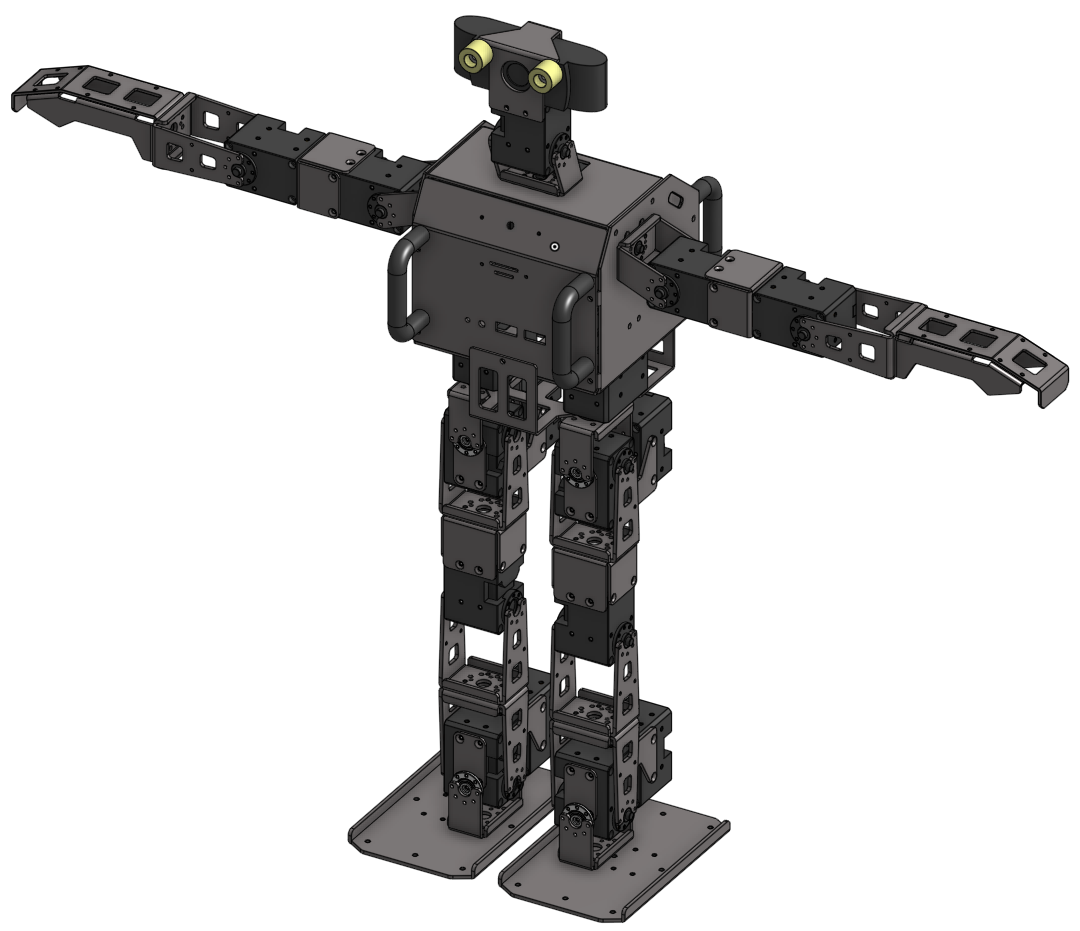
\includegraphics[width=0.45\textwidth]{images/robotis_op3.png}
    \captionsource{Robotis-OP3}{\cite{robotis_op3}}
    \label{fig:robotis_op3}
\end{figure}

\begin{figure}[H]
    \centering
    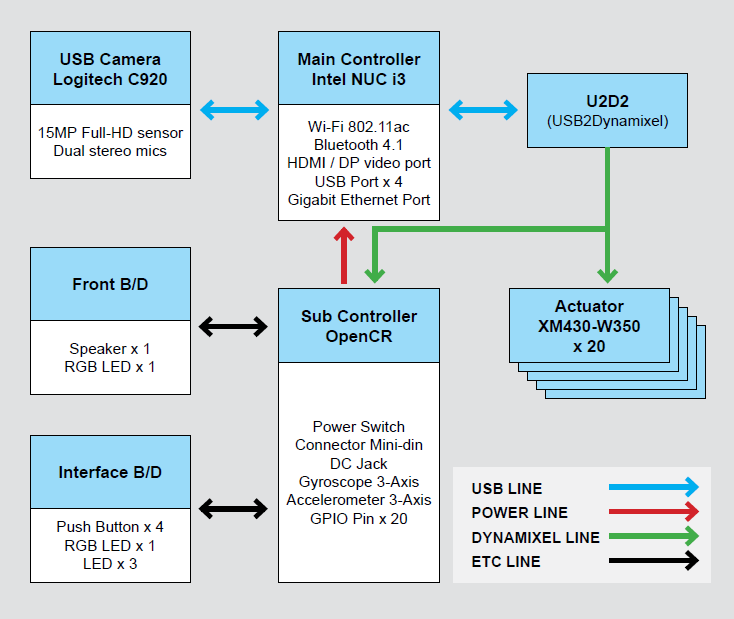
\includegraphics[width=0.6\textwidth]{images/op3_system.png}
    \captionsource{Sistem Robotis-OP3}{\cite{robotis_op3}}
    \label{fig:system_op3}
\end{figure}

\subsection{Dynamixel}

\textit{Dynamixel} adalah aktuator pintar yang dikembangkan oleh Robotis dan banyak digunakan pada sistem robotika modular, termasuk pada robot \textit{humanoid} seperti ROBOTIS-OP3. Berbeda dengan servo konvensional, Dynamixel memiliki fitur komunikasi dua arah yang memungkinkan pengguna tidak hanya mengendalikan sudut atau kecepatan, tetapi juga membaca data seperti posisi saat ini, beban, suhu, dan status error secara real-time \cite{robotis_dynamixel}.

Dynamixel menggunakan protokol komunikasi serial berbasis \textit{half-duplex} dengan dua metode utama, yaitu \textit{TTL} dan \textit{RS-485}. Pada ROBOTIS-OP3, komunikasi dengan servo dilakukan menggunakan protokol \textit{RS-485}, yang mendukung transmisi data jarak lebih jauh dan lebih stabil dibandingkan \textit{TTL}. Setiap servo dihubungkan secara daisy-chain melalui satu jalur komunikasi, sehingga memudahkan perakitan dan pengendalian banyak motor secara simultan \cite{robotis_manual}.

Untuk memudahkan integrasi dengan berbagai bahasa pemrograman, Robotis menyediakan \textit{Dynamixel SDK}, sebuah pustaka perangkat lunak yang mendukung pengendalian servo menggunakan bahasa C, C++, Python, Java, dan MATLAB. SDK ini memungkinkan pengiriman instruksi dan pembacaan data melalui API yang kompatibel dengan berbagai sistem operasi seperti Windows, Linux, dan macOS \cite{robotis_sdk}.

Pada platform ROBOTIS-OP3, terdapat dua jenis seri Dynamixel yang digunakan, yaitu XM430-W350-R dan 2XL430-W250-T. Dynamixel XM430-W350-R digunakan pada bagian kaki dan lengan robot karena memiliki torsi yang cukup besar serta mendukung berbagai mode kontrol seperti posisi, kecepatan, dan arus. Selain itu, motor ini juga dilengkapi dengan fitur \textit{current-based position control} yang memungkinkan pengendalian lebih presisi dan aman terhadap beban berlebih. Sementara itu, Dynamixel 2XL430-W250-T digunakan pada bagian kepala untuk menggerakkan dua sumbu sekaligus, yaitu \textit{yaw} dan \textit{pitch}, dalam satu modul motor. Modul ini memiliki dua port keluaran motor, sehingga lebih efisien dalam penggunaan ruang dan bobot, serta cocok untuk aplikasi di bagian kepala robot yang memerlukan mekanisme gerak ganda dengan dimensi yang lebih ringkas \cite{robotis_op3}.

\begin{figure}[H]
    \centering
    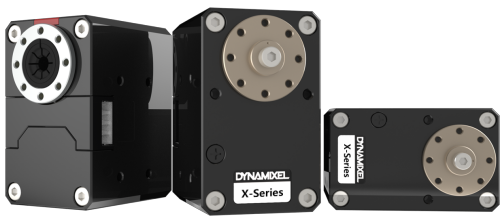
\includegraphics[width=0.6\textwidth]{images/dynamixel.png}
    \captionsource{Dynamixel X-Series}{\cite{robotis_dynamixel}}
    \label{fig:dynamixel}
\end{figure}


\subsection{\textit{Robot Operating System}}
\textit{Robot Operating System} (ROS) adalah \textit{framework} perangkat lunak untuk robotika yang menyediakan berbagai \textit{library} dan alat untuk memfasilitasi pengembangan aplikasi robot. ROS memungkinkan komunikasi antar modul perangkat keras dan perangkat lunak melalui arsitektur berbasis \textit{publish-subscribe} yang efisien, sehingga memudahkan integrasi berbagai komponen seperti sensor, aktuator, dan algoritma kontrol. Selain itu, ROS juga mendukung simulasi gerakan robot menggunakan platform seperti Gazebo, yang memungkinkan pengujian algoritma secara virtual sebelum diimplementasikan pada perangkat keras sebenarnya \cite{sa2024pengembangan}. Pada robot humanoid seperti ROBOTIS-OP3, ROS digunakan untuk berbagai fungsi, termasuk kontrol gerakan, visualisasi data sensor, pengolahan gambar, dan integrasi sistem secara keseluruhan, sehingga menjadi salah satu elemen kunci dalam pengembangan aplikasi robotik.

\subsection{Visi Komputer}
Visi Komputer adalah cabang ilmu komputer yang berfokus pada pengembangan algoritma dan teknik untuk memungkinkan komputer memahami dan mengekstrak informasi bermakna dari data visual seperti gambar, video, atau aliran data dari sensor visual lainnya. Bidang ini bertujuan untuk mensimulasikan kemampuan penglihatan manusia sehingga komputer dapat mengenali, menganalisis, dan membuat keputusan berdasarkan data visual \shortcite{marpaung2022computer}. Teknik dasar dalam visi komputer meliputi deteksi tepi, segmentasi objek, pengenalan fitur, dan estimasi pose. Deteksi tepi digunakan untuk menemukan batasan objek dalam gambar dengan mengidentifikasi perubahan intensitas yang signifikan, seperti yang dilakukan oleh algoritma \textit{Canny Edge Detection}. Segmentasi objek membagi gambar menjadi bagian-bagian yang lebih kecil atau objek tertentu untuk analisis lebih lanjut, menggunakan metode seperti \textit{thresholding} atau \textit{neural networks}. Pengenalan fitur bertujuan untuk mengekstrak elemen-elemen khas seperti sudut, garis, atau pola, yang penting untuk pelacakan atau pengenalan objek. Estimasi pose adalah proses menentukan posisi dan orientasi tubuh manusia atau objek dalam ruang 2D atau 3D, yang biasanya menggunakan algoritma berbasis jaringan saraf tiruan atau model regresi.


Dalam robotika, visi komputer memainkan peran penting dalam berbagai aplikasi. Salah satunya adalah navigasi robot, di mana data visual digunakan untuk mengenali lingkungan sekitar dan menentukan jalur optimal. Selain itu, deteksi lingkungan memungkinkan robot untuk mengidentifikasi rintangan atau area tertentu, membantu dalam penghindaran tabrakan atau penyelesaian tugas. Visi komputer juga digunakan untuk mengenali gerakan manusia, yang menjadi dasar bagi robot \textit{humanoid} dalam meniru gerakan tersebut. Salah satu penerapannya adalah dalam pemodelan gerakan kompleks, seperti gerakan tari atau aktivitas olahraga, yang membutuhkan analisis koordinasi tubuh secara terus-menerus \shortcite{kim2023human}.


\subsection{\textit{Deep Learning}}
Dalam dunia teknologi saat ini sudah tidak asing lagi dengan \textit{Artificial Intelligence} (AI). Perusahaan besar seperti Google, Microsoft, dan Meta saling berlomba untuk menciptakan \textit{Large Language Model} (LLM) seperti \textit{Gemma, Mistral,} dan \textit{Llama}. LLM merupakan salah satu aplikasi utama dari \textit{Deep Learning}, yang memungkinkan pemodelan teks secara kompleks dengan memahami konteks dan hubungan antar kata dalam skala besar.

\textit{Deep Learning} (DL) atau Pembelajaran Mendalam adalah salah satu cabang dari pembelajaran mesin yang berfokus pada pemodelan abstraksi tingkat tinggi pada data. Hal ini dilakukan dengan menggunakan sekumpulan fungsi transformasi non-linear yang ditata secara berlapis-lapis (\textit{deep neural networks}) dan mendalam \cite{ahmad2017mengenal}. DL sangat baik diterapkan pada \textit{supervised learning}, \textit{unsupervised learning}, \textit{semi-supervised learning}, maupun \textit{reinforcement learning} untuk berbagai aplikasi seperti pengenalan citra, pengenalan suara, klasifikasi teks, dan lainnya.

Model dalam DL pada dasarnya dibangun berdasarkan Jaringan Saraf Tiruan (\textit{Neural Network}), yang risetnya telah berlangsung sejak era 1980-an. Namun, DL baru kembali menjadi populer dengan kemajuan teknologi komputer yang semakin cepat, terutama berkat teknologi \textit{Big Data} seperti Hadoop dan Spark berbasis \textit{multi-node cluster}, serta pemrosesan secara paralel berbasis GPU. Jika suatu jaringan memiliki lebih dari tiga lapisan, maka jaringan tersebut dapat disebut sebagai \textit{Deep Network} \shortcite{cholissodin2020ai}.

DL memanfaatkan algoritma berbasis \textit{backpropagation} untuk mengoptimalkan bobot jaringan. Dalam konteks visi komputer, DL telah digunakan secara luas untuk tugas seperti klasifikasi gambar, deteksi objek, segmentasi, dan estimasi pose manusia. Selain itu, DL juga menjadi tulang punggung bagi pengembangan LLM, yang memungkinkan analisis teks secara kompleks dan menghasilkan teks yang menyerupai bahasa manusia.



\begin{figure}[h!]
    \centering
    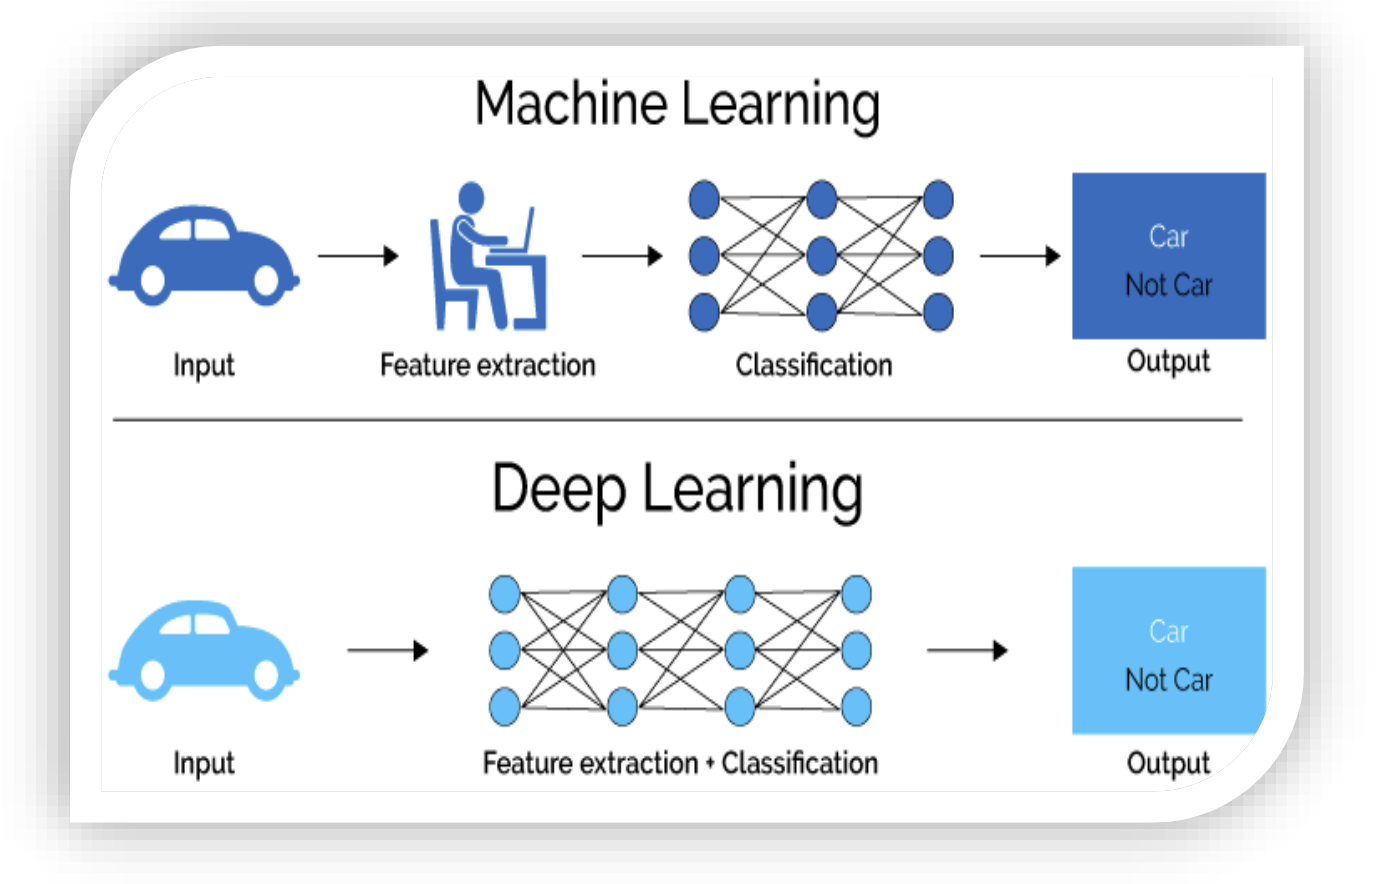
\includegraphics[width=0.5\textwidth]{images/deep_machine_diagram.png}
    \captionsource{Perbedaan ML dan DL}{\cite{cholissodin2020ai}}
    \label{fig:ai_ml_dl_llm}
\end{figure}

\begin{figure}[h!]
    \centering
    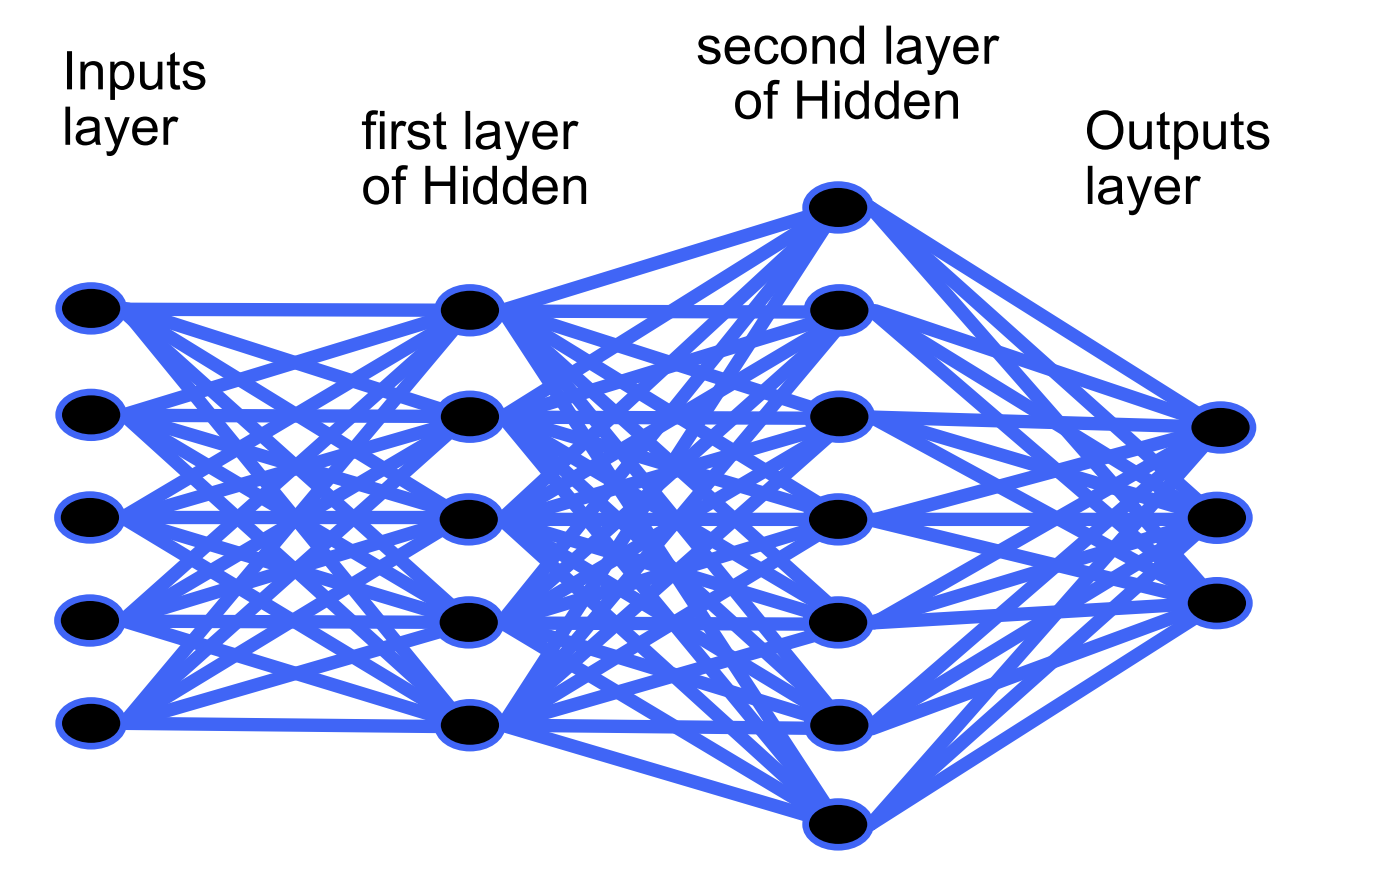
\includegraphics[width=0.5\textwidth]{images/nn.png}
    \captionsource{Ilustrasi Jaringan Saraf Tiruan pada Deep Learning}{\cite{cholissodin2020ai}}
    \label{fig:nn_deeplearning}
\end{figure}


\subsection{\textit{Convolutional Neural Networks} (CNN)}
\textit{Convolutional Neural Networks} (CNN) merupakan arsitektur jaringan saraf tiruan yang dirancang khusus untuk memproses data visual. CNN bekerja dengan mengidentifikasi pola atau fitur dalam gambar melalui operasi konvolusi yang diikuti oleh proses \textit{pooling}. Arsitektur ini menjadi dasar bagi berbagai metode modern dalam tugas-tugas pengenalan citra, deteksi objek, dan estimasi pose manusia.

Salah satu arsitektur CNN yang populer adalah AlexNet. AlexNet diperkenalkan oleh Krizhevsky et al. pada tahun 2012 dan menjadi tonggak penting dalam perkembangan \textit{deep learning} untuk tugas pengenalan citra. Arsitektur ini terdiri dari delapan lapisan, dengan lima lapisan konvolusional diikuti oleh tiga lapisan \textit{fully connected} (FC). AlexNet menggunakan fungsi aktivasi ReLU untuk mempercepat konvergensi pelatihan, serta teknik \textit{dropout} untuk mencegah \textit{overfitting}. Selain itu, AlexNet memperkenalkan penggunaan GPU dalam pelatihan jaringan, yang secara signifikan mempercepat proses komputasi \cite{NIPS2012_c399862d}. 

Keberhasilan AlexNet dalam memenangkan kompetisi \textit{ImageNet Large Scale Visual Recognition Challenge} (ILSVRC) pada tahun 2012 dengan peningkatan akurasi yang signifikan dibandingkan metode sebelumnya menjadikannya model yang mendasari pengembangan arsitektur CNN modern.


\begin{figure}[h!]
    \centering
    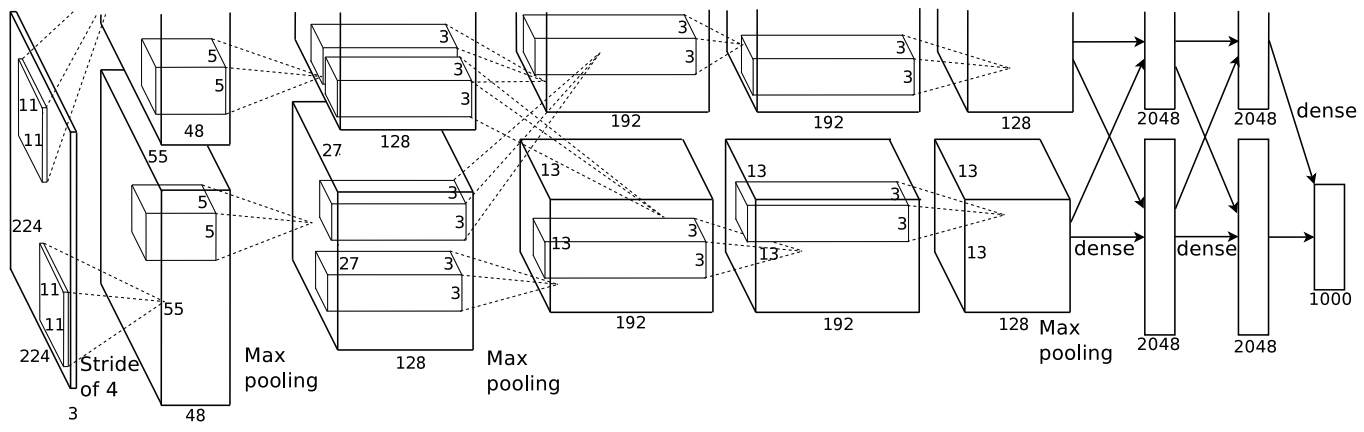
\includegraphics[width=0.9\textwidth]{images/alexnet_architecture.png}
    \captionsource{Arsitektur AlexNet}{\cite{NIPS2012_c399862d}}
    \label{fig:alexnet_architecture}
\end{figure}

\begin{figure}[h!]
    \centering
    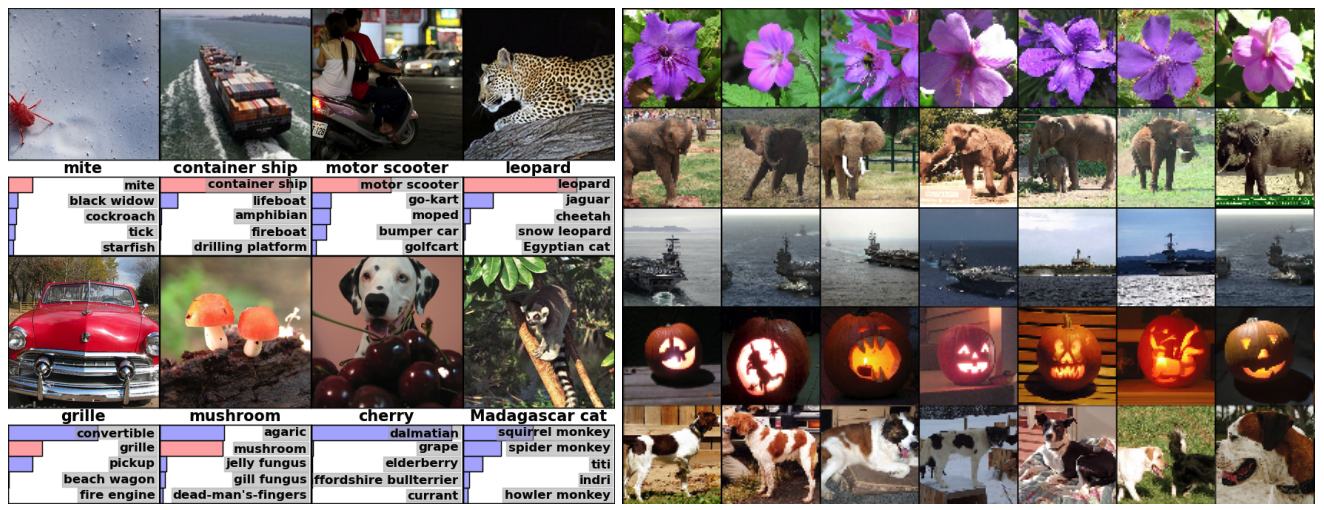
\includegraphics[width=0.9\textwidth]{images/alexnet_result.png}
    \captionsource{Hasil ILSVRC-2010 AlexNet}{\cite{NIPS2012_c399862d}}
    \label{fig:alexnet_result}
\end{figure}

\subsection{\textit{Transformer}}
\textit{Transformer} adalah arsitektur berbasis \textit{attention} yang pertama kali diperkenalkan oleh Vaswani et al. dalam makalah \textit{"Attention Is All You Need"}. Transformers dirancang untuk menggantikan arsitektur tradisional berbasis \textit{recurrent neural networks (RNN)} dan \textit{convolutional neural networks (CNN)} dalam berbagai tugas, khususnya dalam pemrosesan bahasa alami (\textit{natural language processing}, NLP). Keunggulan utama Transformers terletak pada mekanisme \textit{self-attention}, yang memungkinkan model untuk mempelajari hubungan antar elemen dalam data tanpa memerlukan pemrosesan berurutan, seperti pada RNN.

Dalam mekanisme \textit{self-attention}, setiap elemen input dibandingkan dengan elemen lainnya untuk menentukan relevansi antar elemen. Mekanisme ini direpresentasikan dalam bentuk \textit{query}, \textit{key}, dan \textit{value}, di mana relevansi dihitung sebagai nilai dot-product antara \textit{query} dan \textit{key}, yang kemudian digunakan untuk memberikan bobot pada elemen \textit{value} \cite{vaswani2017attention}. Pendekatan ini memungkinkan model untuk memahami hubungan jangka panjang (\textit{long-range dependencies}) dalam data, sehingga cocok untuk data berurutan seperti teks atau video.

\subsection{\textit{Pose Estimation}}
\textit{Pose estimation} adalah proses untuk menentukan lokasi spasial (\textit{keypoints}) tubuh manusia atau objek dalam representasi 2D atau 3D. Proses ini bertujuan untuk mendeteksi titik-titik penting, seperti kepala, siku, lutut, dan pergelangan tangan, yang membentuk kerangka tubuh manusia atau objek. Pada pendekatan modern, jaringan saraf konvolusional (\textit{Convolutional Neural Network}, CNN) digunakan untuk menghasilkan peta panas (\textit{heatmap}) 2D dari input berupa gambar atau video. \textit{Heatmap} ini merepresentasikan probabilitas keberadaan \textit{keypoints} pada setiap piksel gambar \cite{mehta2017vnect}. Untuk menghasilkan pose dalam ruang 3D, peta panas 2D digabungkan dengan informasi tambahan, seperti data kedalaman (\textit{depth}) dari sensor atau rekonstruksi spasial menggunakan teknik regresi koordinat 3D. Pendekatan ini memungkinkan prediksi posisi \textit{keypoints} secara akurat meskipun pada pose yang kompleks atau dalam lingkungan dengan sudut pandang kamera yang tidak ideal.

Saat ini, \textit{pose estimation} telah menjadi salah satu bidang utama dalam visi komputer, dengan berbagai aplikasi mulai dari animasi karakter, pengenalan gerakan manusia, hingga kontrol robot humanoid. Metode berbasis CNN, seperti OpenPose dan HRNet, telah menjadi standar untuk estimasi pose 2D dan 3D dengan akurasi tinggi. Selain itu, arsitektur modern seperti \textit{Transformers} telah diperkenalkan dalam \textit{pose estimation}, misalnya pada model VitPose. Pendekatan berbasis \textit{Transformers} ini menggunakan mekanisme \textit{self-attention} untuk menangkap hubungan spasial dan temporal antara \textit{keypoints}, sehingga menghasilkan prediksi pose 3D yang lebih stabil dan akurat, terutama untuk data video \shortcite{xu2022vitpose}. Keunggulan \textit{Transformers} terletak pada kemampuannya untuk mempelajari konteks yang lebih luas dari data visual, membuatnya ideal untuk tugas yang memerlukan pemahaman gerakan berurutan, seperti dalam penelitian ini yang berfokus pada gerakan tari tradisional Indonesia.

\subsection{MeTRAbs}
MeTRAbs (\textit{Metric-Scale Truncation-Robust Heatmaps for Absolute 3D Human Pose Estimation}) adalah metode yang digunakan untuk memperkirakan pose 3D manusia secara langsung dari gambar RGB, bahkan ketika sebagian tubuh tidak terlihat sepenuhnya dalam gambar. Berbeda dengan metode sebelumnya yang hanya bisa memperkirakan posisi relatif antar sendi tubuh, MeTRAbs mampu memprediksi posisi setiap sendi dalam satuan meter bukan hanya piksel pada gambar.

Metode ini menggunakan representasi \textit{heatmap} 3D, yaitu peta probabilitas untuk setiap titik sendi, yang dibuat dalam ruang tiga dimensi. Semua sumbu dari \textit{heatmap} ini menggunakan skala metrik (meter), bukan piksel, sehingga hasilnya lebih realistis. Jaringan yang digunakan dalam MeTRAbs adalah jaringan konvolusional yang umum digunakan pada visi komputer, seperti ResNet-50, tanpa bagian tambahan yang rumit.

Selain memprediksi posisi 3D relatif antar sendi, MeTRAbs juga dapat memperkirakan posisi absolut tubuh manusia dalam ruang kamera. Ini dilakukan dengan cara menggabungkan prediksi posisi 3D dengan prediksi posisi 2D pada gambar, lalu menghitung posisi tubuh secara keseluruhan menggunakan rumus dari model kamera. Proses ini dilakukan secara otomatis dalam jaringan, sehingga pelatihan bisa dilakukan secara menyeluruh dan efisien.


\begin{figure}[h!]
    \centering
    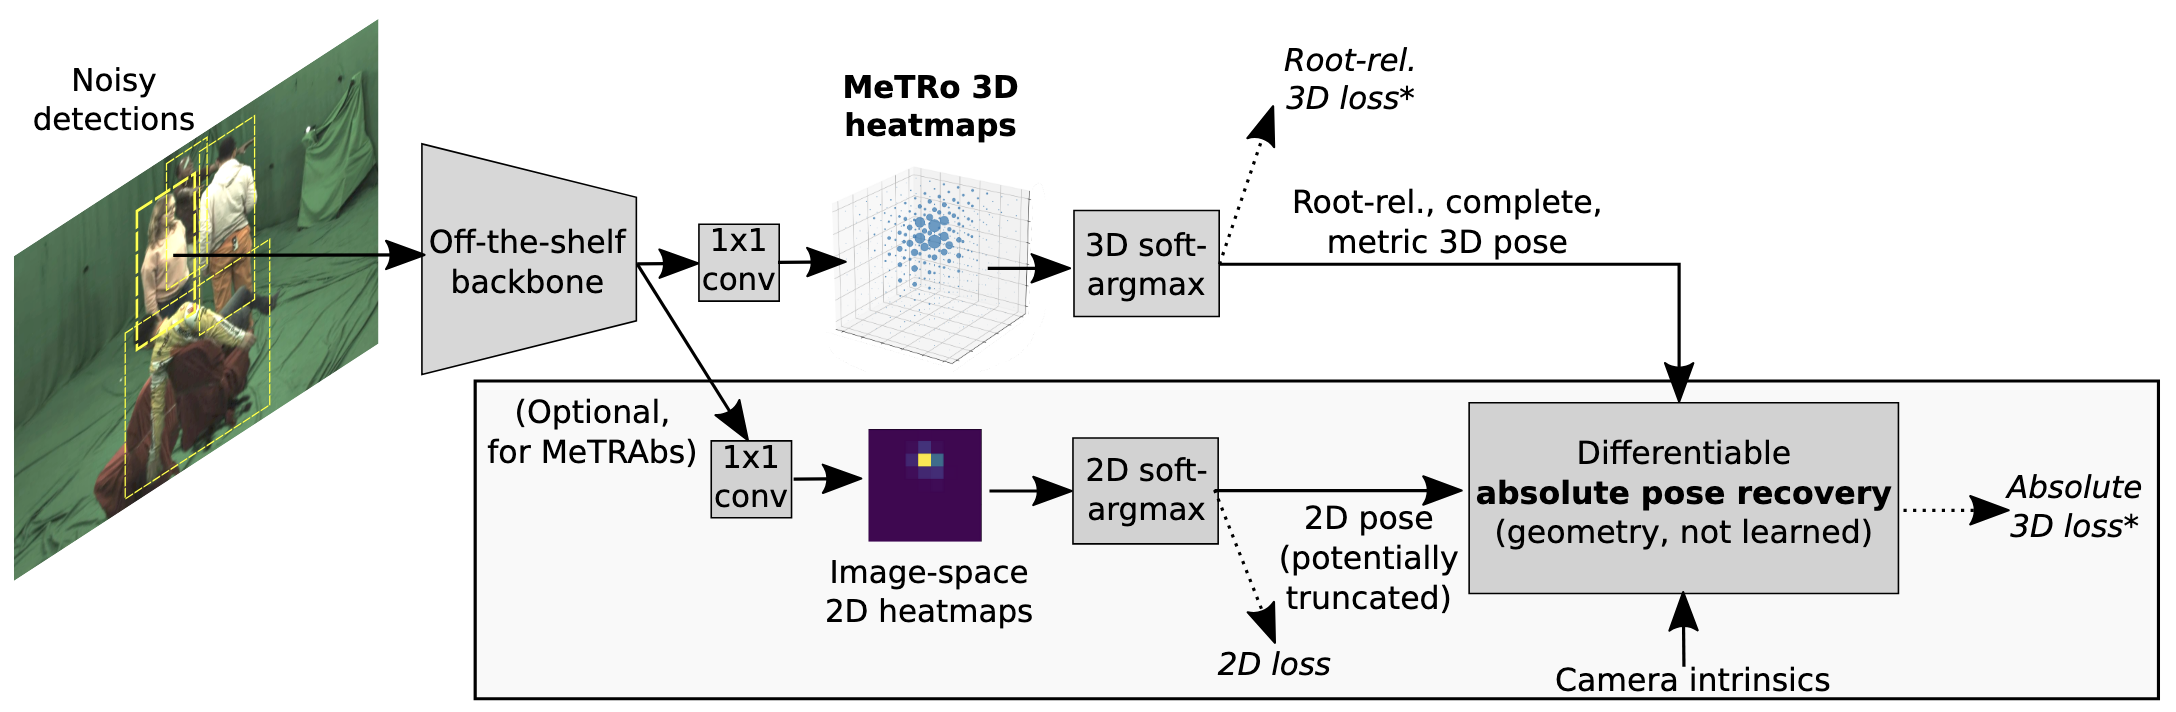
\includegraphics[width=\textwidth]{images/metrabs_architecture.png}
    \captionsource{Arsitektur jaringan MeTRAbs}{\cite{Sarandi2021metrabs}}
    \label{fig:metrabs_architecture}
\end{figure}

Keunggulan MeTRAbs adalah kemampuannya untuk tetap memberikan hasil estimasi yang baik meskipun gambar hanya menampilkan sebagian tubuh saja seperti pada Gambar~\ref{fig:metrabs_architecture}. Selain itu, metode ini tidak memerlukan informasi tambahan seperti panjang tulang atau jarak ke kamera saat pengujian.

\begin{figure}[h!]
    \centering
    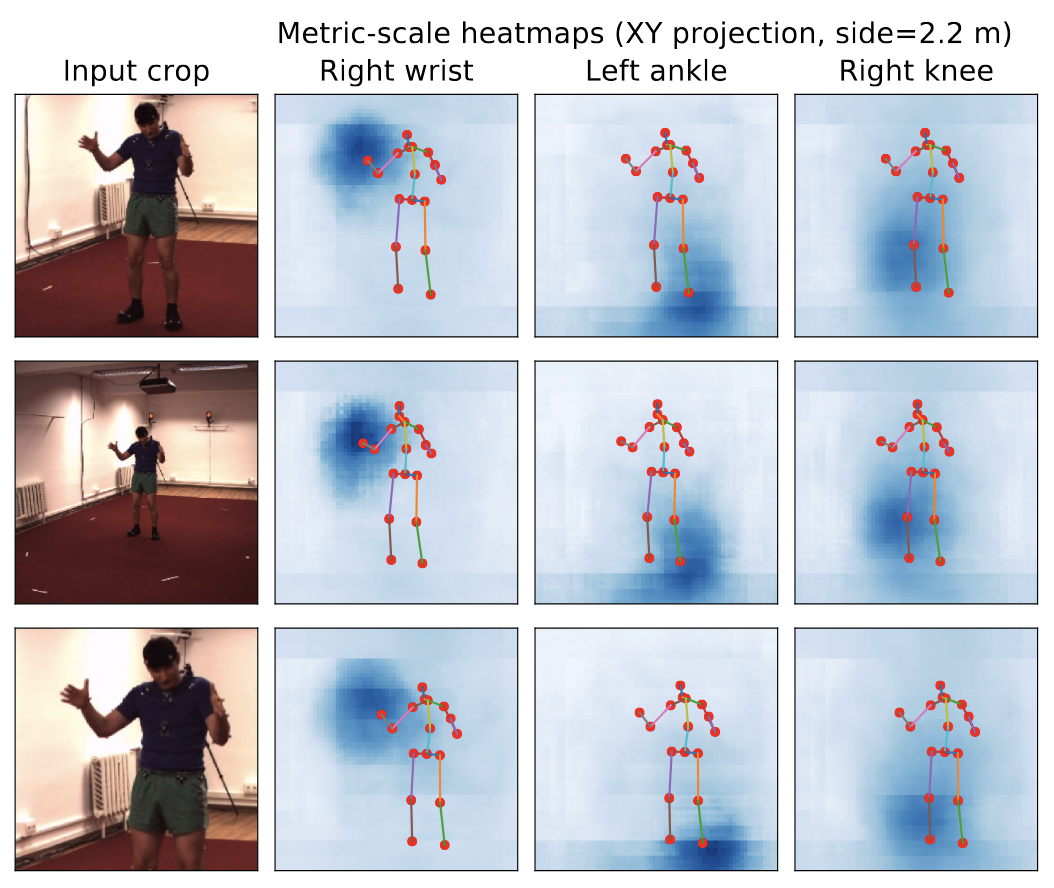
\includegraphics[width=0.6\textwidth]{images/metrabs_result.png}
    \captionsource{Keunggulan MeTRAbs}{\cite{Sarandi2021metrabs}}
    \label{fig:metrabs_result}
\end{figure}

\subsection{DeciWatch}

DeciWatch adalah sebuah kerangka kerja efisien yang dikembangkan untuk meningkatkan estimasi pose manusia 2D/3D pada video dengan mengurangi kebutuhan komputasi hingga 10 kali lipat tanpa mengorbankan akurasi~\cite{zeng2022deciwatch}. Alih-alih memproses setiap frame dalam video, DeciWatch hanya mengambil sebagian kecil frame (sekitar 10\%) melalui \textit{uniform sampling}. 

Arsitektur DeciWatch terdiri dari tiga tahap utama, yaitu \textit{sample-denoise-recover}. Pada tahap pertama, beberapa frame video dipilih secara merata. Pose pada frame-frame ini kemudian diperkirakan menggunakan pose estimator yang ada. Namun karena prediksi ini biasanya mengandung \textit{noise}, DeciWatch menggunakan DenoiseNet, sebuah jaringan berbasis \textit{transformer}, untuk membersihkan hasil estimasi dari noise.

Setelah itu, tahap ketiga dilakukan oleh RecoverNet, jaringan \textit{transformer} lain yang bertugas untuk merekonstruksi pose untuk frame-frame yang tidak diamati. RecoverNet memanfaatkan kontinuitas gerakan manusia dalam video untuk memperkirakan pose pada frame yang tidak diproses langsung. Pendekatan ini terbukti efektif dalam menghasilkan estimasi pose yang lebih halus dan konsisten, terutama pada gerakan yang cepat atau kompleks.

Keunggulan utama DeciWatch adalah efisiensinya. Karena hanya sebagian kecil frame yang dianalisis secara penuh, proses inferensi menjadi jauh lebih ringan, dengan konsumsi memori dan waktu komputasi yang lebih rendah. Selain itu, pendekatan ini juga memperhalus hasil estimasi pose karena mengurangi jitter atau getaran antar frame, menjadikannya sangat cocok untuk aplikasi video seperti pelacakan gerak, interaksi manusia-robot, dan pemodelan tari.

Eksperimen yang dilakukan pada berbagai \textit{dataset} termasuk AIST++ menunjukkan bahwa DeciWatch tidak hanya unggul dalam efisiensi, tetapi juga mampu meningkatkan akurasi secara signifikan dibandingkan metode estimasi frame-by-frame. Kemampuannya dalam menangani gerakan cepat dan data dengan noise menjadikannya sangat relevan dalam konteks penelitian ini.

\begin{figure}[H]
    \centering
    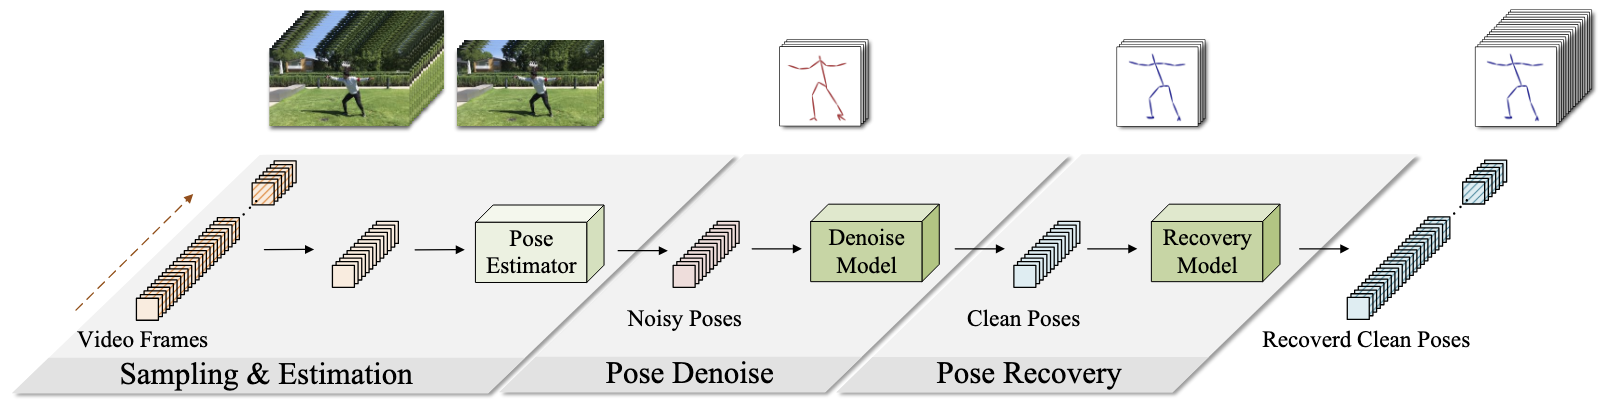
\includegraphics[width=\textwidth]{images/deciwatch_architecture.png}
    \captionsource{Arsitektur DeciWatch}{\cite{zeng2022deciwatch}}
    \label{fig:deciwatch_architecture}
\end{figure}

\subsection{Trigonometri}

Trigonometri adalah cabang matematika yang mempelajari hubungan antara sudut dan panjang sisi dalam segitiga \shortcite{trigono2008maharaj}. Dalam konteks robotika, khususnya pada perhitungan \textit{inverse kinematics}, trigonometri digunakan untuk menentukan sudut artikulasi berdasarkan posisi kartesian dari titik-titik tertentu pada tubuh robot atau manusia. Konsep dasar trigonometri berpusat pada perbandingan sisi dalam segitiga siku-siku, seperti berikut:

\begin{equation}
\sin \theta = \frac{\text{depan}}{\text{miring}}, \quad
\cos \theta = \frac{\text{samping}}{\text{miring}}, \quad
\tan \theta = \frac{\text{depan}}{\text{samping}}
\end{equation}

Pada aplikasi perhitungan sudut dari vektor posisi, fungsi \textit{arctangent} sering digunakan untuk mengubah rasio sisi menjadi sudut. Fungsi ini merupakan kebalikan dari \textit{tangent}, yang mengembalikan nilai sudut \(\theta\) dari rasio \(\frac{y}{x}\). Secara umum, perhitungan sudut menggunakan \textit{arctangent} dapat dituliskan sebagai:

\begin{equation}
\theta = \arctan\left(\frac{y}{x}\right)
\end{equation}

Namun, penggunaan fungsi \(\arctan\) biasa memiliki keterbatasan karena tidak dapat membedakan kuadran dengan benar, sehingga rawan menghasilkan sudut yang salah jika tanda dari \(x\) atau \(y\) berbeda. Untuk mengatasi masalah ini, digunakan fungsi \(\arctan2\), yaitu fungsi khusus yang mempertimbangkan tanda dari \(x\) dan \(y\) secara langsung, sehingga dapat menentukan sudut dengan tepat pada semua kuadran. Notasi umumnya adalah:

\begin{equation}
\theta = \arctan2(y, x)
\end{equation}

Fungsi \(\arctan2\) menghasilkan sudut dalam satuan radian dengan rentang \(-\pi\) hingga \(\pi\), yang sesuai dengan rotasi penuh pada bidang kartesian. Hal ini sangat penting dalam aplikasi robotika untuk memastikan orientasi sudut sesuai dengan posisi aktual vektor di ruang dua dimensi maupun tiga dimensi. Penggunaan trigonometri seperti ini menjadi komponen utama dalam proses \textit{motion retargeting} pada sistem robot humanoid, karena memungkinkan konversi dari data posisi menjadi sudut artikulasi yang dapat dijalankan oleh robot.


\subsection{Matriks Rotasi}

Matriks rotasi adalah alat matematis yang digunakan untuk memutar vektor dalam ruang dua atau tiga dimensi~\shortcite{palazzolo1976rotation}. Dalam bidang robotika, matriks rotasi digunakan untuk mentransformasikan posisi dan orientasi dari satu sistem koordinat ke sistem lainnya, seperti dalam proses \textit{motion retargeting} atau \textit{inverse kinematics}. Rotasi dalam ruang tiga dimensi dapat dinyatakan dengan matriks $3\times3$ untuk masing-masing sumbu utama:

\begin{equation}
R_x(\theta) =
\begin{bmatrix}
1 & 0 & 0 \\
0 & \cos\theta & -\sin\theta \\
0 & \sin\theta & \cos\theta
\end{bmatrix}
\end{equation}

\begin{equation}
R_y(\theta) =
\begin{bmatrix}
\cos\theta & 0 & \sin\theta \\
0 & 1 & 0 \\
-\sin\theta & 0 & \cos\theta
\end{bmatrix}
\end{equation}

\begin{equation}
R_z(\theta) =
\begin{bmatrix}
\cos\theta & -\sin\theta & 0 \\
\sin\theta & \cos\theta & 0 \\
0 & 0 & 1
\end{bmatrix}
\end{equation}

Matriks ini sering digunakan secara berurutan untuk membentuk rotasi gabungan di ruang tiga dimensi sesuai urutan sumbu yang diinginkan. Dalam aplikasi robot humanoid, rotasi ini digunakan untuk mengubah orientasi lengan, kepala, atau bagian tubuh lain sesuai dengan data gerakan manusia.

\subsection{\textit{Inverse Kinematics Transform}}

\textit{Inverse Kinematics Transform} (IKT) adalah metode untuk menghitung sudut-sudut sendi robot berdasarkan posisi titik-titik tubuh manusia, seperti bahu, siku, dan pergelangan tangan, dengan memanfaatkan prinsip geometri dan trigonometri. Pada penelitian \textit{"Robust Regression-Based Motion Perception for Online Imitation on Humanoid Robot"} \shortcite{robust2017imitation}, IKT digunakan untuk mengontrol pergerakan lengan robot humanoid secara langsung dari data pose manusia.

Struktur lengan dianggap sebagai manipulator dua sendi (\textit{two-link manipulator}) dengan empat derajat kebebasan (DOF). Untuk menyederhanakan perhitungan dan mengurangi kompleksitas komputasi, digunakan metode solusi geometris yang bersifat hierarkis dan intuitif. Pendekatan ini lebih efisien dibandingkan metode aljabar karena menghindari solusi yang tidak unik serta mempercepat proses komputasi.

Sebagai contoh, perhitungan sudut pada lengan kiri dilakukan secara bertahap. Pertama, sudut \textit{shoulder pitch} ($\theta_{\text{Pitch}}$) dihitung dari perubahan posisi pada sumbu X dan Z:

\begin{equation}
\theta_{\text{Pitch}} = \arctan2(z_{\text{elbow}} - z_{\text{shoulder}}, x_{\text{elbow}} - x_{\text{shoulder}})
\end{equation}

Kemudian, sudut \textit{shoulder roll} ($\theta_{\text{Roll}}$) dihitung dari perubahan posisi pada sumbu Y terhadap proyeksi vektor lengan atas pada bidang XZ:

\begin{equation}
\theta_{\text{Roll}} = \arctan2(y_{\text{elbow}} - y_{\text{shoulder}}, \sqrt{(x_{\text{elbow}} - x_{\text{shoulder}})^2 + (z_{\text{elbow}} - z_{\text{shoulder}})^2})
\end{equation}

Setelah mendapatkan sudut bahu, vektor lengan bawah diproyeksikan ke sistem koordinat lokal dengan rotasi menggunakan matriks rotasi. Dari situ, sudut \textit{elbow yaw} dan \textit{elbow roll} dihitung dengan prinsip trigonometri serupa. Proses ini memastikan konversi posisi Cartesian menjadi sudut artikulasi dilakukan secara efisien dan dapat berjalan secara \textit{real-time}.

Metode IKT ini sangat sesuai untuk aplikasi \textit{motion retargeting}, karena memungkinkan robot humanoid untuk meniru gerakan manusia secara langsung tanpa proses optimisasi yang berat secara komputasi.


\subsection{\textit{Mean Per Joint Position Error} (MPJPE)}

\textit{Mean Per Joint Position Error} (MPJPE) adalah metrik evaluasi yang umum digunakan dalam estimasi pose manusia 3D. MPJPE mengukur rata-rata jarak Euclidean antara posisi hasil prediksi dan posisi \textit{ground-truth} dari setiap \textit{joint} tubuh manusia dalam ruang 3D. Dengan membandingkan posisi yang diprediksi dengan posisi sebenarnya, MPJPE memberikan gambaran seberapa akurat model memetakan pose manusia~\cite{WANG2021103225}.

Secara matematis, MPJPE dirumuskan sebagai berikut:
\begin{equation}
    E_{\text{MPJPE}}(f, \mathcal{S}) = \frac{1}{N_\mathcal{S}} \sum_{i=1}^{N_\mathcal{S}} \left\lVert P_{f, \mathcal{S}}^{(i)} - P_{gt, f, \mathcal{S}}^{(i)} \right\rVert_2
    \label{eq:mpjpe}
\end{equation}

Pada rumus di atas, \( f \) merepresentasikan satu frame video, dan \( \mathcal{S} \) adalah kerangka tubuh (\textit{skeleton}). \( P_{f, \mathcal{S}}^{(i)} \) merupakan vektor posisi 3D prediksi dari \textit{joint} ke-\( i \), sedangkan \( P_{gt, f, \mathcal{S}}^{(i)} \) adalah posisi 3D dari data \textit{ground-truth}. Nilai \( N_\mathcal{S} \) menyatakan jumlah total \textit{joints}, biasanya sebanyak 17.

Misalkan terdapat 3 titik sendi (\textit{joint}) dengan posisi prediksi dan \textit{ground-truth} berikut:

\begin{itemize}
    \item Joint 1: prediksi = (1, 2, 3), ground-truth = (1, 2, 2)
    \item Joint 2: prediksi = (2, 1, 0), ground-truth = (2, 2, 0)
    \item Joint 3: prediksi = (0, 0, 0), ground-truth = (1, 0, 0)
\end{itemize}

Jarak Euclidean untuk masing-masing joint:
\begin{align*}
    d_1 &= \sqrt{(1{-}1)^2 + (2{-}2)^2 + (3{-}2)^2} = \sqrt{1} = 1 \\
    d_2 &= \sqrt{(2{-}2)^2 + (1{-}2)^2 + (0{-}0)^2} = \sqrt{1} = 1 \\
    d_3 &= \sqrt{(0{-}1)^2 + (0{-}0)^2 + (0{-}0)^2} = \sqrt{1} = 1
\end{align*}

MPJPE = \( \frac{1 + 1 + 1}{3} = 1.0 \) satuan jarak (misal dalam milimeter).

Contoh ini menunjukkan bahwa jika rata-rata kesalahan jarak antara posisi yang diprediksi dan posisi sebenarnya adalah 1 mm, maka MPJPE-nya adalah 1 mm. Nilai MPJPE yang lebih kecil menandakan prediksi pose yang lebih akurat.







